%%%%%%%%%%%%%%%%%%%% author.tex %%%%%%%%%%%%%%%%%%%%%%%%%%%%%%%%%%%
%
% sample root file for your "contribution" to a contributed volume
%
% Use this file as a template for your own input.
%
%%%%%%%%%%%%%%%% Springer %%%%%%%%%%%%%%%%%%%%%%%%%%%%%%%%%%
% RECOMMENDED %%%%%%%%%%%%%%%%%%%%%%%%%%%%%%%%%%%%%%%%%%%%%%%%%%%
\documentclass[graybox]{svmult}
% choose options for [] as required from the list
% in the Reference Guide
\usepackage{type1cm}        % activate if the above 3 fonts are
                            % not available on your system
%
\usepackage{makeidx}         % allows index generation
\usepackage{graphicx}        % standard LaTeX graphics tool
                             % when including Fig.~files
\usepackage{multicol}        % used for the two-column index
\usepackage[bottom]{footmisc}% places footnotes at page bottom
\usepackage{newtxtext}       % 
\usepackage{newtxmath}       % selects Times Roman as basic font
% see the list of further useful packages
% in the Reference Guide
%\makeindex             % used for the subject index
                       % please use the style svind.ist with
                       % your makeindex program
%%%%%%%%%%%%%%%%%%%%%%%%%%%%%%%%%%%%%%%%%%%%%%%%%%%%%%%%%%%%%%%%%%%%%%%%%%%%%%%%%%%%%%%%%
\usepackage{listings, multirow}
\lstset{%
 language={C},
% basicstyle={\scriptsize},%
% identifierstyle={\scriptsize},%
 basicstyle={\small},%
 identifierstyle={\small},%
% commentstyle={\small\itshape},%
%commentstyle={\scriptsize},%
commentstyle={\small},%
 keywordstyle={\small\bfseries},%
 ndkeywordstyle={\small},%
stringstyle={\small\ttfamily},
 frame={tb},
 breaklines=true,
 columns=[l]{fullflexible},%
 numbers=left,%
 xrightmargin=1zw,%
 xleftmargin=1.5zw,%
 numberstyle={\small},%
 stepnumber=1,
 numbersep=1zw,%
% lineskip=-0.1ex%
}
%%%%%%%%%%%%%%%%%%%%%%%%%%%%%%%%%%%%%%%%%%%%%%%%%%%%%%%%%%%%%%%%%%%%%%%%%%%%%%%%%%%%%%%%%
\begin{document}
\title*{Mixed-language programming with XcalableMP}
% Use \titlerunning{Short Title} for an abbreviated version of
% your contribution title if the original one is too long
\author{Masahiro Nakao}
% Use \authorrunning{Short Title} for an abbreviated version of
% your contribution title if the original one is too long
\institute{Masahiro Nakao \at RIKEN Center for Computational Science, 7-1-26 Minatojima-minami-machi, Chuo-ku, Kobe, Hyogo 650-0047, Japan, \email{masahiro.nakao@riken.jp}}
%
% Use the package "url.sty" to avoid
% problems with special characters
% used in your e-mail or web address
%
\maketitle

\abstract*{This chapter shows  linkage functions between XcalableMP and MPI library. Moreover, it  describes how to call XcalableMP program from Python program.}

\abstract{This chapter shows  linkage functions between XcalableMP and MPI library. Moreover, it  describes how to call XcalableMP program from Python program.}

\section{Background}
To develop applications on high-performance computing (HPC) cluster systems,
Partitioned Global Address Space (PGAS) languages that can demonstrate high productivity are used\cite{1303318,Katherine,CGPOP2011,doi:10.1177/1094342017698214}.
Because the use of PGAS languages is familiar in one-sided communication,
applications in PGAS languages can sometimes exhibit higher performance than those using MPI library by directly using a communication layer close to hardware\cite{doi:10.1177/1094342017698214,Jose:2010:UUM:2020373.2020378}. 
Examples of PGAS languages include XcalableMP (XMP)\cite{doi:10.1177/1094342017698214,2013nakao,2012nakao,xmp-spec},
XcalableACC\cite{nakao2014,xacc-spec,nakao2017,nakao2019}, Coarray Fortran\cite{Numrich:1998:CFP:289918.289920}, PCJ\cite{pcj}, Unified Parallel C\cite{upc-1.3},
UPC++\cite{upc_plus_plus}, HabaneroUPC++\cite{Kumar:2014:HCP:2676870.2676879}, X10\cite{Charles:2005:XOA:1103845.1094852},
Chapel\cite{Chamberlain:2007:PPC:1286120.1286123}, and DASH\cite{DBLP:journals/corr/FurlingerFK16}.

Although PGAS languages have many advantages,
re-implementing an existing MPI application using a PGAS language is often not realistic for the following reasons:
(1) since the number of lines of a real-world application code may reach several million, the programming cost for re-implementing is excessive, and
(2) cases where productivity and performance have been improved by PGAS languages are limited.
Moreover, since each programming language generally has its own strong and weak points, it is difficult to develop all parallel applications using just one programming language.

In order to exploit the advantages of a PGAS language,
it is important to consider the linkage between the PGAS language and other languages.
For example,
modifying only a part where the performance or code outlook will be better using a PGAS language
has the potential to partially alleviate the two problems listed in the previous paragraph because the programming cost of partial re-implementation is smaller than that of whole re-implementation.

We have designed an XMP language, and developed Omni compiler described in Chapter 2.
This chapter describes the development of linkage functions between XMP and MPI library for Omni compiler.
Moreover, it also describes how to call XMP program from Python program.
Especially,
since Python has numerous scientific computing libraries,
we believe that linking Python and XMP will lead to a significant reduction in programming cost when developing HPC applications.
%%%%%%%%%%%%%%%%%%%%%%%%%%%%%%%%%%%%%%%%%%%%%%%%%%%%%%%%%%%%%%%%%%%%%%%%%%%%
\section{Translation by Omni compiler}\label{sec:translation}

\begin{figure}[h]
\sidecaption
\includegraphics[scale=.82]{img/translation.eps}
\caption{Example of translation in Omni compiler\cite{pgas-ei}} \label{fig:translation}
\end{figure}

Fig.~\ref{fig:translation} shows an example of a code translation for XMP in C language, where the code of the left figure is translated into that of the right figure
\footnote{Since Omni compiler performs almost the same operation for an XMP in Fortran code, these examples are omitted in this chapter.}.
Omni compiler inserts {\bf xmp\_init\_all()} and {\bf xmp\_finalize\_all()}  automatically  to perform the initialization and finalization processes, respectively.
These functions are defined in Omni compiler runtime library. 
Since  {\bf xmp\_init\_all()} calls  {\bf MPI\_Init()} and {\bf MPI\_Comm\_dup()} internally to duplicate {\bf MPI\_COMM\_WORLD}.
Since the newly duplicated communicator is  used to perform XMP communication,
user MPI communication does not conflict with  XMP communication.
Additionally,  {\bf xmp\_finalize\_all()}  calls  {\bf MPI\_Finalize()} function internally.

In an XMP program,
the \textbf{task} directive can divide a node set.
The implementation of the \textbf{task} directive creates a new communicator based on the duplicated communicator by  {\bf MPI\_Comm\_split()}.
If communication occurs within the range of the \textbf{task} directive,
then the new communicator is used to perform the communication.

Omni compiler renames a user {\bf main()} as  {\bf xmpc\_main()} in order to place the {\bf xmpc\_main()} between  {\bf xmp\_init\_all()} and {\bf xmp\_finalize\_all()}.
New {\bf main()} calls {\bf xmpc\_main()}.
The above special translation is performed only for {\bf main()}.
For other functions (such as {\bf foo()}), renaming is not performed.
%%%%%%%%%%%%%%%%%%%%%%%%%%%%%%%%%%%%%%%%%%%%%%%%%%%%%%%%%%%%%%%%%%%%%%%%%%%%
\section{Functions for mixed-language}
For a mixed-language programming with XMP, Omni compiler has the following functions.

\begin{itemize}
\item Calling an MPI program from an XMP program
\item Calling an XMP program from an MPI program
\item Calling an XMP program from a Python program
\end{itemize}

\subsection{Function to call MPI program from XMP program}\label{sec:MPIfromXMP}
\begin{table}[h]
\centering
\caption{Functions to call MPI program from XMP program\cite{pgas-ei}} \label{tab:MPIfromXMP}
\begin{tabular}{l|l|l|l}
\hline\noalign{\smallskip}
~Language~  & ~Return Value Type~ & ~Function~ & ~Description~ \\ 
\noalign{\smallskip}\svhline\noalign{\smallskip}
~XMP/C      & ~void              & ~xmp\_init\_mpi(int*, char***)~ & \multirow{2}{*}{~Initialize MPI environment}\\
~XMP/F       & ~(None)          & ~xmp\_init\_mpi() & \\  
\noalign{\smallskip}\hline\noalign{\smallskip}
~XMP/C      & ~MPI\_Comm & ~xmp\_get\_mpi\_comm(void) & ~Create MPI communicator from \\
~XMP/F       & ~Integer         & ~xmp\_get\_mpi\_comm() &   ~XMP node set \\
\noalign{\smallskip}\hline\noalign{\smallskip}
~XMP/C      & ~void              & ~xmp\_finalize\_mpi(void) & \multirow{2}{*}{~Finalize MPI environment}\\
~XMP/F       & ~(None)          & ~xmp\_finalize\_mpi() & \\ 
\noalign{\smallskip}\hline\noalign{\smallskip}
\end{tabular}
\end{table}

\begin{figure}[h]
\sidecaption
\includegraphics[scale=.82]{img/program1.eps}
\caption{Example of calling MPI program (mpi.c) from XMP program (xmp.c)\cite{pgas-ei}} \label{fig:program1}
\end{figure}

Table~\ref{tab:MPIfromXMP}  shows  the functions to call an MPI program from an XMP program.
These functions are defined in Appendix A.1 of the XMP specification version 1.4\cite{xmp-spec}.
Fig.~\ref{fig:program1} also shows an example of how to use these functions.
In line 1 of the left figure, an XMP header file (xmp.h) is included to use the functions in Table~\ref{tab:MPIfromXMP}.
In line 2, an MPI header file (mpi.h) is included to obtain the information of the MPI communicator type that is used in line 7.
In line 6,  {\bf xmp\_init\_mpi()} initializes an MPI environment.
In line 8,  {\bf xmp\_get\_mpi\_comm()}  returns an MPI communicator from the information of the executing XMP node set.
In line 9,  {\bf foo()}  which is defined in right figure is called.
In line 10,  {\bf xmp\_finalize\_mpi()}  finalizes the MPI environment.
Note that  {\bf xmp\_get\_mpi\_comm()}  and other MPI functions must be placed between  {\bf xmp\_init\_mpi()} and {\bf xmp\_finalize\_mpi()}.

The implementations of  {\bf xmp\_init\_mpi()} and {\bf xmp\_finalize\_mpi()} are empty because,
as shown in Fig.~\ref{fig:translation},
the {\bf xmp\_init\_all()} and {\bf xmp\_finalize\_all()} are always invoked at the beginning and the end of the program, and these functions initialize and finalize the MPI environment.
Next, an implementation of {\bf xmp\_get\_mpi\_comm()} will be described. 
As shown in section \ref{sec:translation}, the \textbf{task} directive creates a new MPI communicator.
Thus, an MPI communicator is stored at a stack data architecture in Omni compiler runtime library. 
The {\bf xmp\_get\_mpi\_comm()} returns an MPI communicator at the top of the stack.

An example of compilation using Omni compiler is as follows:
\begin{svgraybox}
\$ mpicc mpi.c -c -o mpi.o\\
\$ xmpcc xmp.c -c -o xmp.o \\
\$ xmpcc mpi.o xmp.o -o a.out
\end{svgraybox}

Since Omni compiler uses an MPI compiler as a native compiler internally, MPI programs can also be compiled with the ``xmpcc'' command as follows:
\begin{svgraybox}
\$ xmpcc mpi.c -o mpi.o
\end{svgraybox}

Thus, it is also possible to execute all the compilation work using a single command as follows:
\begin{svgraybox}
\$ xmpcc mpi.c xmp.c -o a.out
\end{svgraybox}

The execution binary is executed using the execution command provided by user's MPI environment as follows:
\begin{svgraybox}
\$ mpirun -np 4 a.out
\end{svgraybox}

%%%%%%%%%%%%%%%%%%%%%%%%%%%%%%%%%%%%%%%%%%%%%%%%%%%%%%%%%%%%%%%%%%%%%%%%%%%%
\subsection{Function to call XMP program from MPI program}
\begin{table}[h]
\centering
\caption{Functions to call XMP program from MPI program\cite{pgas-ei}} \label{tab:XMPfromMPI}
\begin{tabular}{l|l|l|l}
\hline\noalign{\smallskip}
~Language~  & ~Return Value Type~ & ~Function & ~Description \\ 
\noalign{\smallskip}\svhline\noalign{\smallskip}
~XMP/C      & ~void              & ~xmp\_init(MPI\_Comm)~ & \multirow{2}{*}{~Initialize XMP environment~}\\
~XMP/F       & ~(None)          & ~xmp\_init(Integer) & \\ 
\noalign{\smallskip}\hline\noalign{\smallskip}
~XMP/C      & ~void              & ~xmp\_finalize(void) & \multirow{2}{*}{~Finalize XMP environment~}\\
~XMP/F       & ~(None)          & ~xmp\_finalize() & \\ 
\noalign{\smallskip}\hline\noalign{\smallskip}
\end{tabular}
\end{table}

\begin{figure}[h]
\sidecaption
\includegraphics[scale=.82]{img/program2.eps}
\caption{Example of calling XMP program from MPI program\cite{pgas-ei}} \label{fig:program2}
\end{figure}

Table~\ref{tab:XMPfromMPI} shows the functions to call an XMP program from an MPI program.
These functions are defined in Appendix A.2 of the XMP specification version 1.4\cite{xmp-spec}.
Fig.~\ref{fig:program2} shows an example of how to use these functions. 
In line 1 of the left figure,
an XMP header file is included to use functions in the Table \ref{tab:XMPfromMPI}.
In line 7,  {\bf xmp\_init()} initializes an XMP environment,
and creates the XMP node set based on the communicator specified in its argument.
In line 8,
 {\bf foo()}  in the right figure is called.
In line 9,  {\bf xmp\_finalize()} finalizes the XMP environment.
Note that the XMP functions must be placed between  {\bf xmp\_init()} and {\bf xmp\_finalize()}.

Though the {\bf xmp\_init()} is implemented to call the {\bf xmp\_init\_all()} function described in Section \ref{sec:translation},
it also performs the following ingenuities:

\begin{itemize}
\item Before calling {\bf xmp\_init()}, {\bf MPI\_Init()} must be called in the MPI program.
Therefore, we added a procedure that ensures  {\bf MPI\_Init()} is not called in  {\bf xmp\_init\_all()}.
\item As shown in Section \ref{sec:translation},  {\bf xmp\_init\_all()} duplicates {\bf MPI\_COMM\_WORLD} to perform XMP communication.
We also added a procedure that ensures the communicator specified in  {\bf xmp\_init()} is duplicated instead of {\bf MPI\_COMM\_WORLD}.
\end{itemize}

Basically, {\bf xmp\_finalize()} is also implemented to call  {\bf xmp\_finalize\_all()}  in Section \ref{sec:translation}.
As with  {\bf xmp\_init()},
after calling  {\bf xmp\_finalize()}, {\bf MPI\_Finalize()}  is called in an MPI program.
Therefore,
we added a procedure to ensure that  {\bf MPI\_Finalize()} is not called in  {\bf xmp\_finalize\_all()}.

The method to compile and execute is the same as Section \ref{sec:MPIfromXMP}.

\subsection{Function to call XMP program from Python program}
%\begin{table}[h]
%\centering
%\caption{Functions to call XMP program from Python program} \label{tab:XMPfromPython}
%\begin{tabular}{l|l|l}
%\noalign{\smallskip}\hline\noalign{\smallskip}
%~Return Value Type~ & ~Function & ~Description \\ 
%\noalign{\smallskip}\svhline\noalign{\smallskip}
%\multirow{2}{*}{~(None)}  & ~init\_py(ctypes.CDLL, mpi4py.MPI.Intracomm)~ & ~Initialize XMP environment\\
%& ~finalize\_py(ctypes.CDLL) & ~Finalize XMP environment\\
%\noalign{\smallskip}\hline\noalign{\smallskip}
%\end{tabular}
%\end{table}

There are two types of calling an XMP program from a Python program in Omni compiler;
 the one is ``calling from a parallel Python program'', the other is ``calling from a sequential Python program''.

\subsubsection{From parallel Python program}
\begin{figure}[h]
\sidecaption
\includegraphics[scale=.82]{img/program3.eps}
\caption{Example of calling XMP program (bar.c) from parallel Python program (bar.py)\cite{pgas-ei}} \label{fig:program3}
\end{figure}

Fig.~\ref{fig:program3} shows an example of calling an XMP program from a parallel Python program.
We assume the use of ``mpi4py'' for a Python MPI environment.
In line 2 of the left figure, an XMP package is imported which is in Omni compier.
In line 4, the shared library ({\bf bar.so}) created from the right figure is read.
In line 8, {\bf xmp.Lib.call()} calls a parallel XMP program.
This function performs initialization and finalization for an XMP environment internally.

To use the features, the Omni compiler runtime library must be a shared library. 
Therefore, we develop a new compile process to create a shared library for Omni compiler. 
When adding an option ``{\tt {-}{-}enable-shared}'' to ``{\tt ./configure}'' as follows, shared libraries are created.

\begin{svgraybox}
\$ ./configure {-}{-}enable-shared
\end{svgraybox}

An example of compilation and execution using Omni compiler is as follows. 
A shared library is created by ``xmpcc'' command from a user program. 
Compile options used to create the shared library depend on a native compiler (e.g., ``{\tt -fPIC -shard}'' if the native compiler is gcc). 
The execution binary is executed via Python.

\begin{svgraybox}
\$ xmpcc -fPIC -shared bar.c -o bar.so\\
\$ mpirun -np 4 python bar.py
\end{svgraybox}

\subsubsection{From sequential Python program}
\begin{figure}[h]
\sidecaption
\includegraphics[scale=.82]{img/program6.eps}
\caption{Example of spawning XMP program from sequential Python program\cite{pgas-ei}} \label{fig:program6}
\end{figure}
%\begin{figure}[h]
%\sidecaption
%\includegraphics[scale=.82]{img/program4.eps}
%\caption{XMP package in Python (Right) and xmp\_init\_py function (Left)} \label{fig:program4}
%\end{figure}

%The left figure of Fig.~\ref{fig:program4} shows a Python code of the XMP package that defines {\bf init\_py()} and {\bf finalize\_py()}.
%Although the mpi4py can translate an MPI communicator with a Fortran type (MPI\_FINT type) using the {\bf py2f} method, 
%it cannot translate it with a C type.
%Thus,  {\bf init\_py()} first creates the Fortran type MPI communicator,
%after which  {\bf xmp\_init\_py()} defined in the Omni compiler runtime translates it to a C type MPI communicator using {\bf MPI\_Comm\_f2c()}.
%The right figure of Fig.~\ref{fig:program4}  shows the code of {\bf xmp\_init\_py()}.
%The {\bf xmp\_init\_py()} also initializes an XMP environment using  {\bf xmp\_init()} shown in Table~\ref{tab:XMPfromMPI}.

Fig.~\ref{fig:program6} shows an example of calling an XMP program from a sequential Python program.
In line 6, {\bf xmp.Lib.spawn()} calls a parallel XMP program.
The first argument is number of nodes in XMP.
The last argument is an option for asynchronous operation.
If it is true,  processing may return to python before ``{\bf foo()}'' completes.
In line 7, {\bf xmp.Lib.wait()} waits until ``{\bf foo()}'' completes.
In line 9, {\bf xmp.Lib.elapse\_time()} returns  processing time for ``{\bf foo()}''.

An example of execution using Omni compiler is as follows. 
Note that a python program executes with one process, but an XMP program is executed with number of processes specified in code.

\begin{svgraybox}
\$ mpirun -np 1 python bar.py
\end{svgraybox}

%%%%%%%%%%%%%%%%%%%%%%%%%%%%%%%%%%%%%%%%%%%%%%%%%%%%%%%
\section{Application to order/degree problem}
\subsection{What is order/degree program}
The order/degree problem is a problem that minimizes the diameter and average shortest path length (ASPL) among vertices in an undirected graph with a given number of vertices and degrees. 
The problem is useful for designing low latency interconnection networks\cite{graphgolf}.

From the number of vertices ($n$) and degrees ($d$), 
the theoretical lower bounds of the diameter ($K_{n,d}$) and the ASPL ($L_{n,d}$) are calculated as follows\cite{graphgolf,NET:NET3230040405}:

\begin{equation*}
K_{n,d} = \left\{
\begin{array}{ll}
\lceil \frac{n-1}{2} \rceil  & {\rm if}\phantom{a} d = 2 \\[5pt]
\lceil \log_{d-1} (\frac{(n-1)(d-2)}{d}) + 1 \rceil  & {\rm if}\phantom{a} d > 2
%\ceil*{ \frac{n-1}{2}} & {\rm if}\phantom{a} d = 2 \\[5pt]
%\ceil*{ \log_{d-1} (\frac{(n-1)(d-2)}{d}) + 1} & {\rm if}\phantom{a} d > 2
\end{array}
\right.
\end{equation*}

\begin{equation*}
L_{n,d} = \left\{
\begin{array}{ll}
1 & {\rm if}\phantom{a} K_{n,d} = 1 \\
\frac{S_{n,d}+K_{n,d}R_{n,d}}{n-1} & {\rm if}\phantom{a} K_{n,d} \geq 2
\end{array}
\right.
\end{equation*}

\begin{equation*}
S_{n,d} =
\sum_{i=1}^{K_{n,d}-1}  id(d-1)^{i-1} 
\end{equation*}

\begin{equation*}
R_{n,d} = n - 1 - 
\sum_{i=1}^{K_{n,d}-1}  d(d-1)^{i-1} 
\end{equation*}

\begin{figure}[t]
 \begin{minipage}{0.5\hsize}
  \begin{center}
\includegraphics[scale=0.25,clip]{img/n10d3-random.eps}
\caption{Diameter = 3,ASPL = 1.89}\label{fig:example-random}
  \end{center}
 \end{minipage}
 \begin{minipage}{0.5\hsize}
  \begin{center}
\includegraphics[scale=0.25,clip]{img/n10d3-opt.eps}
\caption{Diameter = 2,ASPL =1.67}\label{fig:example-opt}
  \end{center}
 \end{minipage}
\end{figure}

Fig.~\ref{fig:example-random} and Fig.~\ref{fig:example-opt} 
show examples of  graphs with  $n=10$ and $d=3$ and their distance matrices. 
The distance matrix indicates the shortest hop count between vertices. 
The diameter is the maximum value of the elements in the distance matrix. 
ASPL is the value obtained by dividing the total value of all elements by the number of elements $(n^2 - n)/2$. 
While the graph in Fig.~\ref{fig:example-random} has random edges, the graph in Fig.~\ref{fig:example-opt} has edges optimized by our algorithm, 
which is described in section \ref{sec:implementation}. 
The diameter and ASPL of Fig.~\ref{fig:example-opt} are theoretical lower bounds.

\begin{table*}[t]
\centering
\caption{Combination of vertices and degrees of General Graph Category in 2017} \label{tab:syutudai}
\begin{tabular}{r||r|r|r|r|r|r|r|r|r|r}\hline\hline
Number of vertices & 32 & 256 & 576 & 1344 & 4896 & 9344 & 88128 & 98304 & 100,000 & 100,000 \\ \hline
Number of degrees & 5 & 18 & 30 & 30 & 24 & 10 & 12 & 10 & 32 & 64\\ \hline
\end{tabular}
\end{table*}

In an effort to expand the order/degree problem into open science, 
the National Institute of Informatics has held a ``Graph Golf'' competition every year since 2015 to search for the smallest diameter and ASPL. 
A combination of several vertices and degrees is provided in each of those events. 
The competition has two categories: one is the General Graph Category, 
where vertices are placed freely, and the other is the Grid Graph Category, 
where vertices are placed on a two-dimensional grid. 
This section deals with the General Graph Category. 
Table \ref{tab:syutudai} shows the combination of vertices and degrees used in 2017.

A python program ``create-random.py'' for the  order/degree problem is available on the official Graph Golf website\cite{graphgolf}. 
The program outputs follow from the number of vertices and degrees. These calculations use the Python networkx package\cite{networkx}.

\begin{itemize}
\item Initial graph with random edges (the graph of Fig.~\ref{fig:example-random} is created by this function)
\item Calculation of diameter and ASPL 
\item Graph figure in Portable Network Graphics (PNG) format (the graphs shown Fig.~\ref{fig:example-random} and Fig.~\ref{fig:example-opt} are created by this function)
\end{itemize}

\subsection{Implementation}\label{sec:implementation}
The ``create-random.py'' does not search out the smallest diameter and ASPL. 
Moreover, to obtain diameter and ASPL of a graph, 
it is necessary to calculate all of the shortest paths among its vertices.
Although the ``create-random.py'' calculates the shortest paths using the {\bf shortest\_path\_length} method of the networkx package,
this method requires a significant amount of time.

\begin{figure}[t]
\centering
\includegraphics[scale=0.55,clip]{img/flow.eps}
\caption{Flow chart of an algorithm in Python and XMP/C} \label{fig:flow}
\end{figure}

To search for the smallest diameter and ASPL, 
we developed a GraphGolf code in both Python and XMP/C based on ``create-random.py.'' 
A Simulated Annealing (SA)\cite{Metropolis1953, Kirkpatrick671} algorithm is used for optimization. 
The shortest paths calculation is parallelized by XMP directives. 
Fig.~\ref{fig:flow} shows a flow chart for the algorithm. 
While Python is used to create initial graph and output the figure, 
XMP/C is used to implement other parts.

\begin{figure}[t]
\begin{lstlisting}
import ctypes
import xmp 
import networkx as nx
import argparse

argumentparser = argparse.ArgumentParser()
argumentparser.add_argument('vertex', type=int)
argumentparser.add_argument('degree', type=int)
vertex = args.vertex
degree = args.degree

arr = ((c_int * 2) * (vertex * degree / 2 + 1))()
arr[i][0] = vertex
arr[i][1] = degree
for i, l in enumerate(nx.generate_edgelist(g, data=False)):
    arr[i+1][0] = int(l.split()[0])
    arr[i+1][1] = int(l.split()[1])

lib = xmp.Lib("xmp_graphgolf.so")
lib.spawn(4, "xmp_graphgolf", arr, async = False)

image_name = "n"+str(vertex)+"d"+str(degree)+".png"
lines = []
for line in arr:
    lines.append(str(line[0]) + " " + str(line[1]))
    G = nx.parse_edgelist(lines, nodetype = int)
    save_image(G, image_name)

def save_image(g, filepath):
    import matplotlib as mpl
    mpl.use('Agg')
    import matplotlib.pyplot as plt
    layout = nx.circular_layout(g)
    nx.draw(g, with_labels=False, node_size=50, linewidths=0, alpha=0.5, node_color='#3399ff', edge_color='#666666', pos=layout)
    plt.draw()
    plt.savefig(filepath)
        
\end{lstlisting}
\caption{Code in Python} \label{fig:program-python}
\end{figure}

\begin{figure}[t]
\begin{lstlisting}
#pragma xmp template t[:]
#pragma xmp nodes p[*]
#pragma xmp distribute t[block] onto p

void xmp_graphgolf(int *edge)
{
    :
int vertices = edge[0];
#pragma xmp template_fix t[vertices]
#pragma xmp loop on t[i]
  for(int i=0;i<vertices;i++){
    :  // Calculate diameter and ASPL
    }
#pragma xmp reduction(+:ASPL)
#pragma xmp reduction(max:diameter)
  :
}
\end{lstlisting}
\caption{Code in XMP/C} \label{fig:program-xmp}
\end{figure}


Fig.~\ref{fig:program-python} and  Fig.~\ref{fig:program-xmp} show a portion of our codes.
In lines 6-10 of Fig.~\ref{fig:program-python}, 
the number of vertices and degrees are transformed to allow their use in the program. 
In lines 12-17, an initial graph is created and set a variable {\it arr}. 
The first element of the variable {\it arr} stores the number of vertices and the degree.
In lines 19-20, 
the initial graph is passed to the {\bf xmp\_graphgolf} function of Fig.~\ref{fig:program-xmp}, which optimizes it. 
The result is saved in a variable {\it arr}, 
which is the same as one of the arguments. 
After  line 22, the result is transformed into a figure. 
In lines 1-3 of Fig.~\ref{fig:program-xmp}, 
the XMP directives declare the template and node set, 
and then distributes the template onto the node set in a block manner. 
In line 1, the ``[:]'' means that the template size is not fixed at this point. 
In line 9, the \textbf{template\_fix} directive determines the template size {\it vertices}, which is the number of vertices. 
In lines 11-13, a diameter and ASPL are calculated. The calculation is a state of the ``Compute energy'' shown in Fig.~\ref{fig:flow}. 
This calculation uses the top-down approach of the breadth-first search.
%The calculation order for the shortest path of all vertexes is $O(n^2d)$. 
In line 10, the {\bf loop} directive parallelizes the loop statement to calculate each shortest path in parallel. In lines 14-15, 
the {\bf reduction} directives aggregate a diameter and ASPL stored at each node.

\subsection{Evaluation}
\begin{table}[t] 
\renewcommand{\arraystretch}{1.2}
\centering
\caption{Coma system specifications} \label{tab:coma}
\begin{tabular}{l|l}\hline \hline
CPU & Intel Xeon-E5 2670v2 2.5 GHz 10 Cores x 2 Sockets \\
Memory & DDR3 1866MHz 59.7GB/s 64GB \\
Network & InfiniBand FDR 7GB/s \\
\multirow{2}{*}{Software} & intel/16.0.2, intelmpi/5.1.1, Omni compiler 1.2.1 \\
& Python 2.7.9, networkx 1.9\\ \hline
\end{tabular}
\end{table}

To evaluate the performance of the Graph Golf application, 
we used the ``coma'' system located in University of Tsukuba, the specifications of which are shown in Table \ref{tab:coma}. 

\begin{figure}[t]
\centering
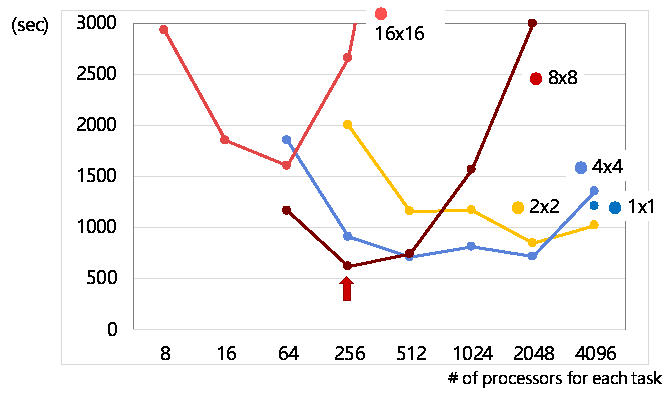
\includegraphics[scale=0.55,clip]{img/result.eps}
\caption{Performance evaluation} \label{fig:result}
\end{figure}

We measured the time required to calculate all of the shortest paths once by changing the number of nodes.
We assigned 20 XMP nodes to each compute node, and used
a medium-sized number of vertices and degrees ($n = 9344$, $d = 10$), as shown in Table \ref{tab:syutudai}.

Fig.~\ref{fig:result} shows performance results where the bar graph shows the time measurements, 
and the line graph shows the parallel efficiency of one XMP node.
The time for one XMP node is 123.17 seconds, 
while the time for 1,280 XMP nodes (using 64 compute nodes) is 0.13 seconds, 
which is 921 times faster. 
Since the time using the Python networkx package is 148.83 seconds in one CPU core, 
XMP achieved a performance improvement of 21\%.

\begin{figure}[t]
\centering
\includegraphics[scale=0.55,clip]{img/comm.eps}
\caption{Calculation and communication ratio}\label{fig:comm}
\end{figure}

From an examination of Fig.~\ref{fig:result}, we found that the parallel efficiency decreases as the number of nodes increases. 
We consider that the following reasons are responsible for the decrease:

\begin{itemize}
\item The ratio of communication time increases. 
Fig.~\ref{fig:comm} shows the ratio of communication time and calculation time to the total time. 
As the number of nodes increases, the proportion of communication time also increases.
\item The parallelized loop lengths are non-uniform. 
The length of the loop statement in line 11 of Fig.~\ref{fig:program-xmp} is 9,344, 
which is the same as the number of vertices. 
Since the length is divided by the number of nodes, 
the length non-uniformity increases as the number of nodes increases.
%For example, even if the communication time is 0 using 1,280 XMP nodes, 
%the maximum parallel efficiency becomes 0.91 (= $9344/(\lceil 9334/1280 \rceil/1280)$).
%Since the length is divided by the number of nodes,
%each node has eight indices at the maximum ( $\lceil 9334/1280 \rceil = 8$).
%As the number of nodes increases, the length non-uniformity increases.
%For example,
%even if the communication time is 0 using 1,280 nodes, 
%the maximum parallel efficiency becomes 0.91 (= $9344/(8/1280)$).
\end{itemize}

\section{Conclusion}
This chapter describes how to use  linkage functions between XMP and MPI library in Omni compiler. 
Moreover, it  also describes how to call  an XMP program from a Python program.
Users can call functions written in these languages with a simple procedure.
Since many existing parallel applications are written in MPI library, these functions can be useful for extending existing applications.
Furthermore, it will be possible to effectively use the high functionality of Python.

%%%%%%%%%%%%%%%%%%%%%%%%%%%%%%%%%%%%%%%%%%%%%%%%%%%%%%%%%%%%%%%%%%%%%%%%%%%%
%%%%%%%%%%%%%%%%%%%%%%%% referenc.tex %%%%%%%%%%%%%%%%%%%%%%%%%%%%%%
% sample references
% %
% Use this file as a template for your own input.
%
%%%%%%%%%%%%%%%%%%%%%%%% Springer-Verlag %%%%%%%%%%%%%%%%%%%%%%%%%%
%
% BibTeX users please use
% \bibliographystyle{}
% \bibliography{}
%

\begin{thebibliography}{99.}%
% and use \bibitem to create references.
%
% Use the following syntax and markup for your references if 
% the subject of your book is from the field 
% "Mathematics, Physics, Statistics, Computer Science"
%
% Contribution 
\bibitem{caf} Robert W. Numrich and John Reid, ``Co-Array Fortran for
		parallel programming'', ACM SIGPLAN Fortran Forum, Vol.~17,
		No.~2 (1998).
\bibitem{upc} UPC Consortium, ``UPC Specifications, v1.2'', Lawrence
		Berkeley National Lab (LBNL-59208) (2005).
\bibitem{chapel} David Callahan, Bradford L.~Chamberlain and Hans
		P.~Zima,  ``The Cascade High Productivity Language'', Proc. 9th
		Int'l. Workshop on High-Level Parallel Programming Models and
		Supportive Environments (HIPS 2004), pp.~52--60 (2004).

\bibitem{ompt}
		{OpenMP Architecture Review Board}, ``OpenMP Application
		Programming Interface Version 5.0'' (2018).


\bibitem{MUST-project}
{The MUST Project},
\newblock https://www.itc.rwth-aachen.de/must.

\bibitem{Extrae-project}
{The Extrae Project},
\newblock https://tools.bsc.es/extrae.
%
% \bibitem{pro-env} Programming Environment Research Team.
% \url{https://pro-env.riken.jp}
% %
% \bibitem{hpcs} High Performance Computing System laboratory, University of Tsukuba, Japan.
% \url{https://www.hpcs.cs.tsukuba.ac.jp}
% %
% \bibitem{xcodeml} Mitsuhisa Sato et al.
%   ``Omni Compiler and XcodeML: An Infrastructure for Source-to-Source Transformation'',
%   Platform for Advanced Scientific Computing Conference (PASC16), Lausanne, Switzerland, Jun. (2016)
%  %
% \bibitem{ixpug} Masahiro Nakao et al.
%   ``Performance Evaluation for Omni XcalableMP Compiler on Many-core Cluster System based on Knights Landing'',
%   IXPUG Workshop Asia 2018, Tokyo, Japan, Jan. pp. 52--58 (2018)
% %
% \bibitem{github} \url{https://github.com/omni-compiler/omni-compiler}
% %
% %\bibitem{guide} \url{https://omni-compiler.org/manual/en/}
% %
% \bibitem{gasnet} \url{https://gasnet.lbl.gov}
% %
% \bibitem{scalasca} \url{https://www.scalasca.org}
% %
% \bibitem{hpcc} \url{https://icl.utk.edu/hpcc/}
% %
% \bibitem{hpca} Masahiro Nakao et al.
% ``Implementation and evaluation of the HPC Challenge benchmark in the XcalableMP PGAS language'',
%   International Journal of High Performance Computing Applications, 33(1), 110-123. Mar. (2017)
% %
% \bibitem{hpcc-a} \url{https://www.hpcchallenge.org}%
% %
% \bibitem{blas} BLAS: Basic Linear Algebra Subprograms \url{http://www.netlib.org/blas/} (2016)
% %
% \bibitem{fft1} David H. Bailey.
%   ``FFTs in external or hierarchical memory. Journal of Supercomputing'',
%   Vol.4, pp.23--35 (1990)
% %
% \bibitem{fft2} Van Loan C.
%   ``Computational Frameworks for the Fast Fourier Transform'',
%   Society for Industrial and Applied Mathematics (1992)
% %
% \bibitem{ffte} Daisuke Takahashi.
%   A Fast Fourier Transform Package. \url{http://www.ffte.jp} (2014)
% %
% \bibitem{randomaccess} Ponnusamy R. et al.
%   ``Communication overhead on the CM5: an experimental performance evaluation'',
%   Fourth Symposium on the Frontiers of Massively Parallel Computation, pp.108--115 (1992)
% %
% \bibitem{modified} HPL Algorithm Panel Broadcast. \url{http://www.netlib.org/benchmark/hpl/algorithm.html} (2016)
% %
% %\bibitem{XACC1} Masahiro Nakao et al.
% %  ``XcalableACC: Extension of XcalableMP PGAS Language Using OpenACC for Accelerator Clusters'',
% %  Proceedings of the First Workshop on Accelerator Programming Using Directives, pp.27--36 (2014)
% %
% %\bibitem{XACC2} Masahiro Nakao et al.
% %  ``Evaluation of XcalableACC with Tightly Coupled Accelerators/InfiniBand Hybrid Communication on Accelerated Cluster'',
% %  International Journal of High Performance Computing Applications, Jan. (2019)
% %
% %\bibitem{caf-hpcc} Guohua Jin et al.
% %  ``Implementation and Performance Evaluation of the HPC Challenge Benchmarks in Coarray Fortran 2.0'',
% %  Parallel Distributed Processing Symposium (IPDPS), 2011 IEEE International, pp.1089--1100 (2011)
% %
% %\bibitem{2012Chapel-HPCC} Brad Chamberlain et al.
% %  ``Chapel HPC Challenge Entry'',
% %  \url{http://www.hpcchallenge.org/presentations/sc2012/ChapelHPCC2012.pdf} (2011)
% %
% %\bibitem{2012X10-HPCC} Olivier Tardieu et al.
% %  ``X10 for Productivity and Performance at Scale'',
% %  \url{http://www.hpcchallenge.org/presentations/sc2012/x10-hpcc.pdf} (2012)
% %
% %\bibitem{Tardieu:2014:XAP:2555243.2555245} Olivier Tardieu et al.
% %  ``X10 and APGAS at Petascale'',
% %  Proceedings of the 19th ACM SIGPLAN Symposium on Principles and Practice of Parallel Programming pp.53--66 (2014)
% %
% %\bibitem{Kennedy:2007:RFH:1238844.1238851} Kennedy Ken et al.
% %  ``The rise and fall of High Performance Fortran: an historical object lesson'',
% %  Proceedings of the third ACM SIGPLAN conference on History of programming languages, pp.7-1--7-22 (2007)
% %
% %\bibitem{tsugane2016} Keisuke Tsugane et al.
% %  ``Proposal for Dynamic Task Parallelism in PGAS Language XcalableMP'',
% %  The 6th AICS International Symposium, p.57 (2016)
\end{thebibliography}

\end{document}
